\documentclass{article}

\usepackage{fancyhdr, lastpage}
\usepackage[inline]{enumitem}
\usepackage{listings}
\usepackage[scaled=0.95]{inconsolata}  % Use a monospaced font, like Inconsolata
\usepackage{wasysym}
\usepackage{booktabs}
\usepackage{booktabs, multicol, multirow, array, threeparttable}
\usepackage{siunitx}
\usepackage{xfrac}
\usepackage{extramarks}
\usepackage{amsmath, amsthm, amsfonts, mathtools, empheq}
\usepackage{caption}
\usepackage[table]{xcolor}
\usepackage{tikz}
\usepackage[most]{tcolorbox}
\usepackage{pagecolor} %% for dark background
\usepackage{hyperref}
\usepackage{refcount}
\usepackage{subfigure}

\topmargin=-0.45in
\evensidemargin=0in
\oddsidemargin=0in
\textwidth=6.5in
\textheight=9.0in
\headsep=0.25in

\linespread{1.1}

% Define a command to print last page number without hyperlink
\newcommand*{\lastpagewithoutlink}{%
    \getpagerefnumber{LastPage}%
}

\pagestyle{fancy}
\lhead{\hmwkAuthorName}
\chead{\hmwkTitle}
\rhead{\hmwkClass}
\lfoot{\lastxmark}
\cfoot{Page \thepage \ of \lastpagewithoutlink}


\renewcommand\headrulewidth{0.4pt}
\renewcommand\footrulewidth{0.4pt}

\setlength\parindent{0pt}

%
% Create Problem Sections
%

\newcommand{\enterProblemHeader}[1]{
    \nobreak\extramarks{}{Problem \arabic{#1} continued on next page\ldots}\nobreak{}
    \nobreak\extramarks{Problem \arabic{#1} (continued)}{Problem \arabic{#1} continued on next page\ldots}\nobreak{}
}

\newcommand{\exitProblemHeader}[1]{
    \nobreak\extramarks{Problem \arabic{#1} (continued)}{Problem \arabic{#1} continued on next page\ldots}\nobreak{}
    \stepcounter{#1}
    \nobreak\extramarks{Problem \arabic{#1}}{}\nobreak{}
}

\setcounter{secnumdepth}{0}
\newcounter{partCounter}
\newcounter{homeworkProblemCounter}
\setcounter{homeworkProblemCounter}{1}
\nobreak\extramarks{Problem \arabic{homeworkProblemCounter}}{}\nobreak{}

%
% Homework Problem Environment
%
% This environment takes an optional argument. When given, it will adjust the
% problem counter. This is useful for when the problems given for your
% assignment aren't sequential. See the last 3 problems of this template for an
% example.
%
\newenvironment{homeworkProblem}[1][-1]{
    \ifnum#1>0
        \setcounter{homeworkProblemCounter}{#1}
    \fi
    \section{Problem \arabic{homeworkProblemCounter}}
    \setcounter{partCounter}{1}
    \enterProblemHeader{homeworkProblemCounter}
}{
    \exitProblemHeader{homeworkProblemCounter}
}

%
% Homework Details
%   - Title
%   - Due date
%   - Class
%   - Section/Time
%   - Instructor
%   - Author
%

\newcommand{\hmwkTitle}{Homework\ \#5}
\newcommand{\hmwkDueDate}{May 5th, 2024}
\newcommand{\hmwkClass}{EGR 5110}
\newcommand{\hmwkClassTime}{}
\newcommand{\hmwkClassInstructor}{Professor Nissenson}
\newcommand{\hmwkAuthorName}{\textbf{Francisco Sanudo}}

%
% Title Page
%

\title{
    \vspace{2in}
    \textmd{\textbf{\hmwkClass:\ \hmwkTitle}}\\
    \normalsize\vspace{0.1in}\small{Due\ on\ \hmwkDueDate\ at 11:59pm}\\
    \vspace{0.1in}\large{\textit{\hmwkClassInstructor\ \hmwkClassTime}}
    \vspace{3in}
}

\author{\hmwkAuthorName}
\date{}

\renewcommand{\part}[1]{\textbf{\large Part \Alph{partCounter}}\stepcounter{partCounter}\\}

%
% More settings
%

% Define MATLAB code style
\lstdefinestyle{matlabstyle}{%
  language=Matlab,
  basicstyle=\ttfamily\small,    % Use a smaller font
  keywordstyle=\color{blue},
  commentstyle=\color{green!40!black},
  stringstyle=\color[RGB]{167, 9, 245},
  numbers=left,
  numberstyle=\tiny,
  numbersep=5pt,
  frame=single,
  breaklines=true,
  breakatwhitespace=true,
  captionpos=b,
  morekeywords={matlab2tikz},
  showstringspaces=false,
}

\newcommand{\mat}[1]{\lstinline[style=matlabstyle]|#1|}

% Table Settings
% \setlength{\tabcolsep}{5pt} % Gap before text starts
\renewcommand{\arraystretch}{2.5} % Cell Height Scaling
\setlength{\arrayrulewidth}{0.5mm} % Table Border Thickness
\arrayrulecolor{blue} % Table Border Color
\newcolumntype{s}{>{\columncolor{black!10}} c}

% Link Settings
\hypersetup{
    colorlinks=false,       % false: boxed links; true: colored links
    linkcolor=red,          % color of internal links (change box color with linkbordercolor)
    citecolor=green,        % color of links to bibliography
    urlcolor=cyan,           % color of external links
    pdftitle={EGR 5110 HW3}
}

% Color defintions
\definecolor{magenta}{RGB}{255,0,255}
\definecolor{cyan}{RGB}{0,255,255}
\definecolor{white}{RGB}{255,255,255}
\definecolor{red}{RGB}{255,0,0}
\definecolor{green}{RGB}{0,255,0}
\definecolor{orange}{RGB}{255,165,0}
\definecolor{yellow}{RGB}{255,255,0}
\definecolor{blue}{RGB}{10,10,255}

% Text color shortcuts
\newcommand{\cw}{\color{white}}
\newcommand{\cm}{\color{magenta}}
\newcommand{\cc}{\color{cyan}}
\newcommand{\cred}{\color{red}}
\newcommand{\cb}{\color{blue}}
\newcommand{\cg}{\color{green}}
\newcommand{\cy}{\color{yellow}}
\newcommand{\co}{\color{orange}}

%
% Various Helper Commands
%


% For derivatives
\newcommand{\deriv}[2]{\frac{d#1}{d#2}}

% For partial derivatives
\newcommand{\pderiv}[2]{\displaystyle \frac{\partial #1}{\partial #2}}

% Redefine \dfrac if you want all fractions to be in display style automatically
\newcommand{\ddfrac}[2]{\frac{\displaystyle #1}{\displaystyle #2}}

% Alias for the Solution section header
\newcommand{\solution}{\textbf{\large Solution}}

%% Box settings
% \setlength{\fboxsep}{9pt} % Adjust the padding thickness here
\setlength{\fboxrule}{1pt} % Adjust the border thickness here

% The \dimexpr\linewidth-2\fboxsep-2\fboxrule\relax calculation ensures that the width of the minipage is reduced by twice the padding and twice the border width, as there is padding and border on both the left and right sides.
\newcommand{\boxsettings}{\dimexpr\linewidth-2\fboxsep-2\fboxrule\relax}

% Paragraph box shortcut for tables
\newcommand{\PB}[2]{\parbox{#1}{\centering #2}}

%% make subscripts smaller
% \begingroup\lccode`~=`_
% \lowercase{\endgroup\def~}#1{_{\scriptscriptstyle#1}}
% \AtBeginDocument{\mathcode`_="8000 \catcode`_=12 }

%% small negative sign
\newcommand{\dashexp}{\scalebox{0.35}[0.5]{$-$}}
\newcommand{\dash}{\scalebox{0.5}[1.0]{$-$}}


\begin{document}

\maketitle

\pagebreak

\tableofcontents

\pagebreak

\section{Background}
Homework \#5 required the construction of a numerical integrator using quadratic splines to calculate the area under a general set of data points that could be unevenly spaced. \\

Given the following set of inputs:
\begin{enumerate}
    \item \mat{x} -- Time vector corresponding to velocity data
    \item \mat{fx} -- Velocity vector
    \item \mat{tinstant} -- Time at which to determine the instantaneous velocity
    \item \mat{t1 & t2} -- Initial and final times for distance calculations
\end{enumerate}

The numerical integrator was expected to return the following outputs:
\begin{enumerate}
    \item \mat{totaldist} -- Total distance traveled from the beginning to the end of the time vector
    \item \mat{vinstant} -- Instantaneous velocity at the specified time \mat{tinstant}
    \item \mat{subdist} -- Distance traveled between the specified times \mat{t1} and \mat{t2}
\end{enumerate}

\section{Testing The Integrator}

To assess the validity of the integrator, it's important to test it against a function with a known analytical solution. Consider the following quadratic function:
\begin{equation}
    f(x) = x^2
    \label{eq:quad}
\end{equation}

Integrating from $x_1$ to $x_2$ yields:
\begin{align*}
    \begin{split}
        \int_{x_1}^{x_2} x^2 & = \left.\frac{1}{3} x^3\right|_{x_1}^{x_2} \\
                             & = \frac{1}{3} x_2^3 - \frac{1}{3} x_1^3
    \end{split}
\end{align*}

For example, let's test the integrator using the following:
\begin{lstlisting}[style=matlabstyle, caption = {Integrator Inputs}]
x = [1 2 6 7 10 13 20 25];      % Time vector
fx = x.^2;                      % Velocity vector
tinstant = 8;                   % Instantaneous velocity query time
t1 = 3;                         % Start time for distance calculation
t2 = 14;                        % End time for distance calculation
\end{lstlisting}

Integrating \eqref{eq:quad} over the entire time range (1 to 25 seconds) yields:
\begin{equation*}
    \int_{1}^{25} x^2 = \frac{1}{3} 25^3 - \frac{1}{3} 1^3 = 5208
\end{equation*}

Integrating \eqref{eq:quad} over the subset time range (3 to 14 seconds) yields:
\begin{equation*}
    \int_{3}^{14} x^2 = \frac{1}{3} 14^3 - \frac{1}{3} 3^3 = 905.6667
\end{equation*}

The velocity at \mat{tinstant} (8 seconds) is:
\begin{equation*}
    f(8) = 8^2 = 64 
\end{equation*}

\pagebreak

\section{Numerical Integration Accuracy}
The implementation of the quadratic spline integrator introduces several important considerations and potential sources of discrepancy when computing the integral of a velocity function over specified intervals. One primary consideration is the accuracy of numerical integration methods employed in the code. The integrator utilizes quadratic splines to approximate the velocity function between data points. However, the accuracy of this approximation relies on the number of spline segments ($N$) and the degree of the polynomial used. With quadratic splines, while providing a reasonable approximation, the method might not capture rapid changes in the velocity function accurately, particularly over larger intervals. In addition, error is expected because we assume the second derivative is 0 at the first data point, making the first spline a line instead of curve. \\

The following shows the output from the numerical integrator:
\begin{lstlisting}[style=matlabstyle, caption = {Integrator Output},numbers=none, label={lst:output}]
>> [totaldist,vinstant,subdist] = quadspline(x,fx,tinstant,t1,t2)

totaldist =

       5210.1


vinstant =

        64.03


subdist =

       907.27
\end{lstlisting}

The results shown in Listing~\ref{lst:output} indicate that the numerical solution aligns very closely to the analytical one, with some small error. Compared to the analytical solution, \mat{totaldist} is within 0.04\%, \mat{vinstant} is within 0.04\%, while \mat{subdist} fell within 0.17\%. For the given set of data points, the integrator showed great performance but could be improved by introducing a larger set of data points (i.e., increasing the number of quadratic spline segments), or emplying higher-order polynomial approximations (e.g. cubic splines) if necessary.\\

Figure~\ref{fig:fig1} depicts the quadratic spline fit performed on the given set of data points.

\pagebreak

\begin{figure}[h]
    \centering
    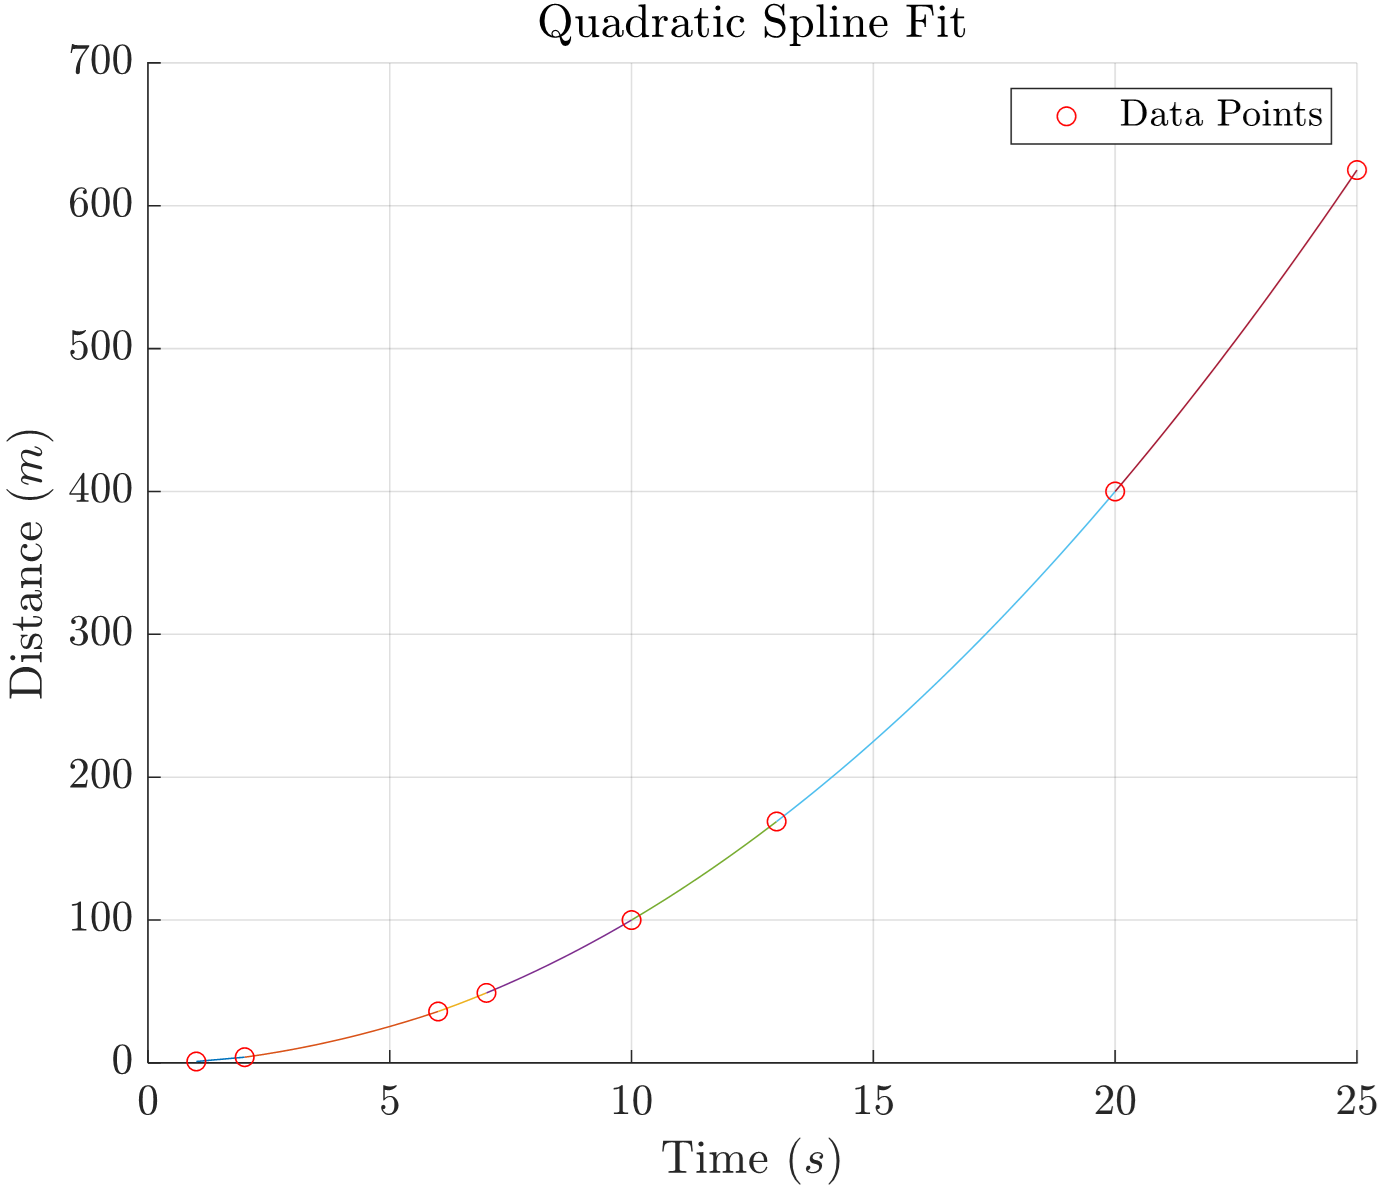
\includegraphics[width=0.8\textwidth]{fig/quadSplineFit.png}
    \caption{Quadratic Spline Interpolation Between Data Points}
    \label{fig:fig1}
\end{figure}

\pagebreak

\section{Quadratic Spline Integrator -- MATLAB Code}

\lstinputlisting[
  style=matlabstyle,
  caption={Quadratic Spline Integrator}
]{../code/quadspline.m}

\end{document}
